\begin{frame}{Montagem e conferência dos componentes}
  \begin{columns}[c,onlytextwidth]
    \begin{column}{0.46\textwidth}
      \centering
      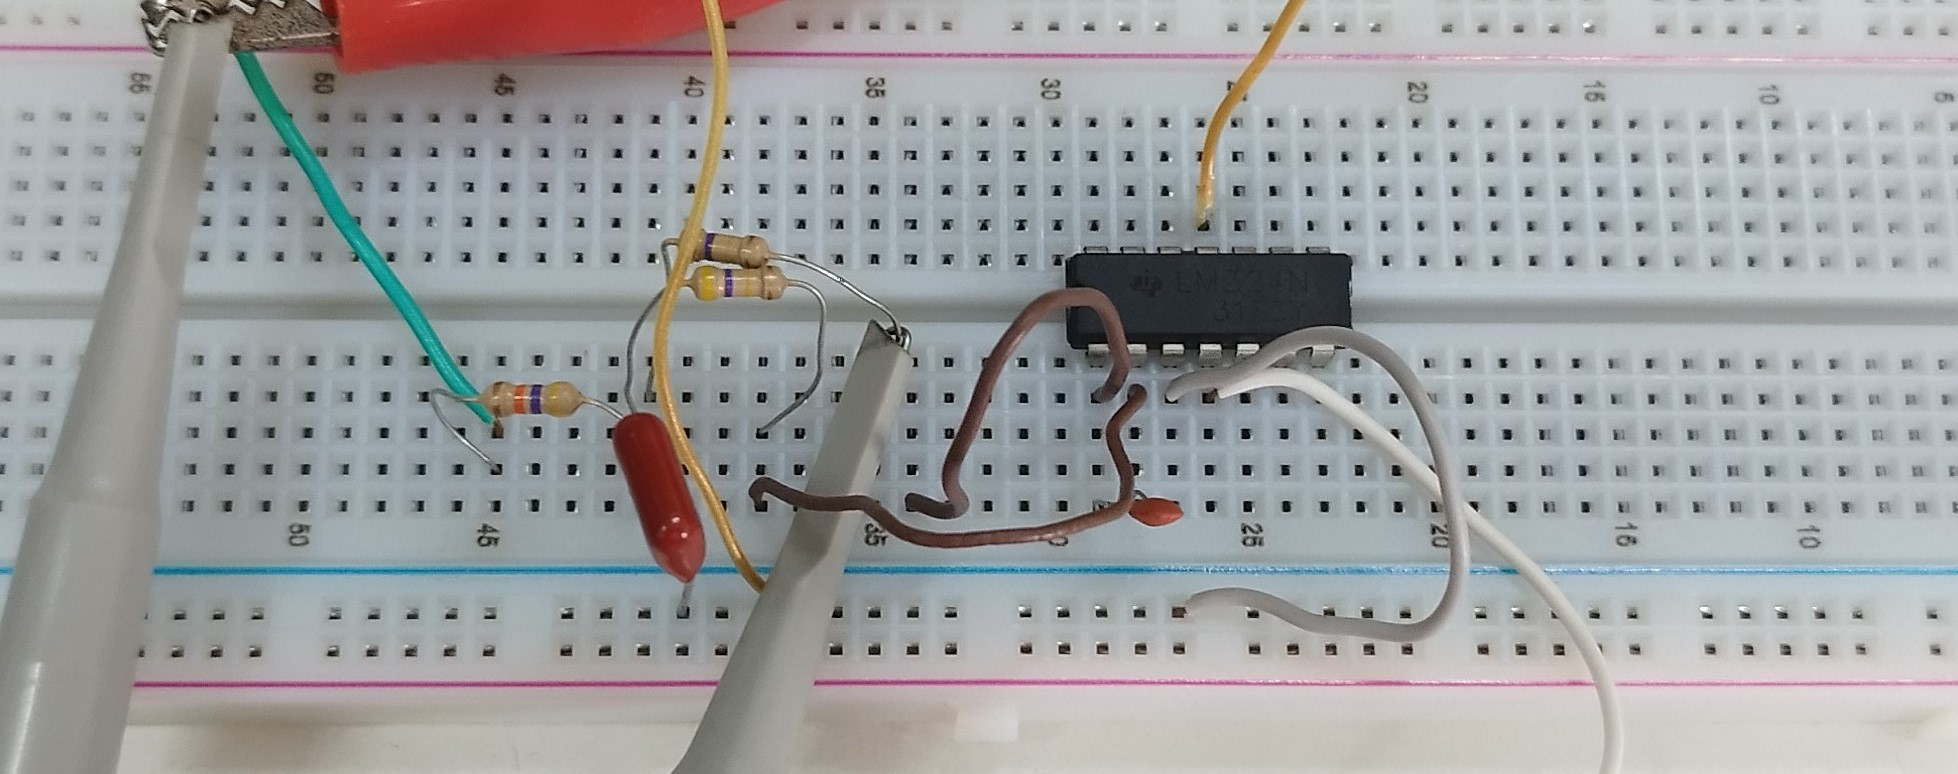
\includegraphics[width=\linewidth]{slides/img/montagem_protoboard.jpg}

      \vspace{0.10cm}
      \scriptsize Montagem em protoboard: acervo da prática.

      \begin{block}{Instrumentação}
        \small Fonte simétrica, multímetro, gerador de sinais e osciloscópio
        para observar entrada e saída.
      \end{block}
    \end{column}
    \begin{column}{0.51\textwidth}
      \centering
      \small
      \textbf{Valores registrados no relatório}

      \vspace{0.12cm}
      \renewcommand{\arraystretch}{1.16}
      \begin{tabular}{lcc}
        \toprule
        Componente & Nominal & Medido \\
        \midrule
        $C_1$ & $100\,\mathrm{nF}$ & $109{,}9\,\mathrm{nF}$ \\
        $C_2$ & $10\,\mathrm{nF}$ & $11{,}42\,\mathrm{nF}$ \\
        $R_1$ & $470\,\mathrm{k}\Omega$ & $469{,}4\,\mathrm{k}\Omega$ \\
        $R_2$ & $470\,\mathrm{k}\Omega$ & $478{,}0\,\mathrm{k}\Omega$ \\
        $R_3$ & $47\,\mathrm{k}\Omega$ & $47{,}13\,\mathrm{k}\Omega$ \\
        \bottomrule
      \end{tabular}

      \vspace{0.16cm}
      \scriptsize A identificação dos resistores nesta tabela corresponde ao
      circuito 2. As curvas teóricas desta apresentação usam os valores nominais.
    \end{column}
  \end{columns}
\end{frame}
